%!TEX program = xelatex
\documentclass{beamer}

\usepackage{blindtext}

\usetheme{Execushares}

\title{{\Large False positives detection in connectomics\\ through hierarchical sparsity}}
\subtitle{matteo.frigo@epfl.ch}
\author{Matteo Frigo}
\date{INRIA Sophia Antipolis - 19th May 2017}

\usepackage{amsmath,amssymb,amsfonts,amsthm}
%\usepackage{empheq}
\usepackage{bigints}
\usepackage{bookmark}
\usepackage{emptypage}
\usepackage{graphicx} %\includegraphics{figura.ext}
\usepackage{epstopdf} % per includere immagini .eps
%\usepackage[dvipsnames]{xcolor}
\usepackage{subfigure}
\usepackage{quoting}
\usepackage{listings}
%\usepackage{enumerate}
%\usepackage{enumitem}
\usepackage{datetime}
\usepackage{etoolbox}
\usepackage{wasysym}
%\usepackage{epigraph}
\usepackage{pgf,tikz}
\usepackage{mathrsfs}
\usetikzlibrary{arrows}
\definecolor{qqzzqq}{rgb}{0.,0.6,0.}
\definecolor{ffqqqq}{rgb}{1.,0.,0.}
\definecolor{qqqqff}{rgb}{0.,0.,1.}
\definecolor{mygreen}{rgb}{0.0, 0.5, 0.0}
\usepackage{mathtools}
\usepackage{verbatim}
\usepackage{textcomp}

%\usepackage{fourier} % font figo
%\usepackage{euler}
%\usepackage[math]{iwona}
%\usepackage[varg]{txfonts}
%\usepackage{microtype}
%\usepackage[colorinlistoftodos]{todonotes}
%\usepackage{latexsym}
%\usepackage{lmodern}

\DeclareMathOperator{\Prox}{\mathbf{prox}}
\newcommand{\prox}[2]{\Prox_{#1}\left({#2}\right)}
\DeclareMathOperator*{\argmin}{argmin}
\newcommand{\NN}{\mathbb{N}}
\newcommand{\ZZ}{\mathbb{Z}}
\newcommand{\QQ}{\mathbb{Q}}
\newcommand{\RR}{\mathbb{R}}
\newcommand{\rd}{\mathbb{R^d}}
\newcommand{\CC}{\mathbb{C}}
\newcommand{\norm}[1]{\left\|{#1}\right\|}
\newcommand{\normtwosq}[1]{\norm{#1}_2^2}
\newcommand{\onehalf}{\frac{1}{2}}
\newcommand {\matlab} {$\text{Matlab}^{\circledR}$\,}
\newcommand {\expect} {\mathbb{E}}
\newcommand {\prob} {\mathbb{P}}
\renewcommand{\epsilon}{\varepsilon}
%\renewcommand{\theta}{\vartheta}
%\renewcommand{\rho}{\varrho}
\renewcommand{\phi}{\varphi}
\hyphenation{sub-dif-fe-ren-tial}

\newcommand<>{\uncoverubrace}[2]{%
  \onslide#3 \underbrace{ \onslide<1->%
  #1%
  \onslide#3 }_{#2} \onslide<1->%
}
\newcommand<>{\uncoverobrace}[2]{%
  \onslide#3 \overbrace{ \onslide<1->%
  #1%
  \onslide#3 }^{#2} \onslide<1->%
}



\setcounter{showSlideNumbers}{1}
\setcounter{showProgressBar}{1}

\begin{document}


\frame{\titlepage}


\begin{frame}
\frametitle{Joint work with...}
\begin{itemize}
\item Prof. Giandomenico Orlandi
\item Prof. Jean-Philippe Thiran
\item Prof. Alessandro Daducci
\item Muhamed Barakovic
\end{itemize}
\vfill
\begin{center}
\includegraphics[width=.7\textwidth]{img/loghi}
\end{center}

\end{frame}


\begin{frame}
\frametitle{The goal: structural connectivity}
\vfill
\begin{minipage}{.45\textwidth}
\includegraphics[width=\textwidth]{img/fulltract}
\end{minipage}\hfill $\Longrightarrow$ \hfill
\begin{minipage}{.45\textwidth}
\includegraphics[width=\textwidth]{img/connectivitymatrix}
\end{minipage}

\vfill
\begin{center}
\textbf{Quantify the connections within the brain}
\end{center}
\end{frame}


\begin{frame}
\frametitle{The problem: false positives}
\begin{flushleft}
\textbf{Tractography-based connectomes are dominated by false-positive connections}
\end{flushleft}
\begin{flushright}
\emph{Maier-Hein et al., 2016 (bioarxiv)}
\end{flushright}
%\includegraphics[width=.9\textwidth]{img/paperauthors1}

\begin{itemize}
\item 96 distinct tractography pipelines
\item \emph{``most algorithms routinely extracted many false positive bundles''} 
\item \emph{``Tractography identifies more invalid than valid bundles''} 
\item \textbf{\emph{``Tractography is fundamentally ill‐posed''}} 
%\item 2568 downloads since Nov 7th, 2016
\end{itemize}
\end{frame}

\begin{frame}
\frametitle{The problem: false positives}
\begin{flushleft}
\textbf{Connectome sensitivity or specificity: which is more important?}

{\scriptsize \begin{itemize}
\item \emph{``the impact of FPs and FNs on empirical connectomes indicate that specificity is at least twice as important as sensitivity''}
\end{itemize}
}
\end{flushleft}
{\tiny \begin{flushright}
\emph{Zalesky, A. et al., 2016 (NeuroImage)}
\end{flushright}}

\begin{flushleft}
\textbf{Anatomical accuracy of brain connections derived from diffusion MRI tractography is inherently limited}

{\scriptsize \begin{itemize}
\item \emph{``The methods that show the highest sensitivity show the lowest specificity, and vice versa''}
\end{itemize}
}
\end{flushleft}
{\tiny \begin{flushright}
\emph{Thomas, C. et al., 2014 (PNAS)}
\end{flushright}}
\end{frame}

\begin{frame}
\frametitle{Forward model}
\begin{equation}
\nonumber
y = Ax + \epsilon
\end{equation}
Given
\begin{description}
\item[$x$:] vector of weights
\item[$A$:] dictionary for the fibres
\item[$\epsilon$:] systematic+random error
\end{description}
Obtain
\begin{description}
\item[$y$:] acquired dMRI data
\end{description}
\end{frame}

\begin{frame}
\frametitle{Forward model: COMMIT}
\quad \\
\begin{center}
\textbf{{\normalsize Convex Optimisation Modelling\\ for Microstructure Informed Tractography}}
\end{center}
{\tiny \begin{flushright}
\emph{Daducci et al., 2015 (IEEE TMI)}
\end{flushright}}

Input: \\ \quad \\

\begin{minipage}{.3\linewidth}
\begin{center}
Acquired DWI\\
\includegraphics[width=\linewidth]{img/commit/COMMIT_idea_1_var}
\end{center}
\end{minipage}\hfill
\begin{minipage}{.3\linewidth}
\begin{center}
Tractography\\
\includegraphics[width=\linewidth]{img/commit/COMMIT_idea_2_var}
\end{center}
\end{minipage}\hfill
\begin{minipage}{.3\linewidth}
\begin{center}
Microstructure model\\
\includegraphics[width=\linewidth]{img/commit/COMMIT_idea_3_var}
\end{center}
\end{minipage}\hfill
\end{frame}

\begin{frame}
\frametitle{Forward model: COMMIT}
\quad \\ \quad \\
\begin{center}
\begin{minipage}{.3\linewidth}
\begin{center}
\includegraphics[width=\linewidth]{img/commit/COMMIT_idea_1_var}
\end{center}
\end{minipage}\qquad \qquad
\begin{minipage}{.3\linewidth}
\begin{center}
\includegraphics[width=\linewidth]{img/commit/COMMIT_idea_2_var}
\end{center}
\end{minipage}

\includegraphics[width=\linewidth]{img/commit/COMMIT_idea_4}
\end{center}
\end{frame}

\begin{frame}
\frametitle{Forward model: COMMIT}
\quad \\ \quad \\
\begin{center}
\begin{minipage}{.3\linewidth}
\begin{center}
\includegraphics[width=\linewidth]{img/commit/COMMIT_idea_1_var}
\end{center}
\end{minipage}\qquad \qquad
\begin{minipage}{.3\linewidth}
\begin{center}
\includegraphics[width=\linewidth]{img/commit/COMMIT_idea_2_var}
\end{center}
\end{minipage}

\includegraphics[width=\linewidth]{img/commit/COMMIT_idea_5}
\end{center}
\end{frame}

\begin{frame}
\frametitle{Forward model: COMMIT}
\quad \\ \quad \\
\begin{center}
\begin{minipage}{.3\linewidth}
\begin{center}
\includegraphics[width=\linewidth]{img/commit/COMMIT_idea_1_var}
\end{center}
\end{minipage}\qquad \qquad
\begin{minipage}{.3\linewidth}
\begin{center}
\includegraphics[width=\linewidth]{img/commit/COMMIT_idea_2_var}
\end{center}
\end{minipage}

\includegraphics[width=\linewidth]{img/commit/COMMIT_idea_6}
\end{center}
\end{frame}

\begin{frame}
\frametitle{Forward model: COMMIT}
\quad \\ \quad \\
\begin{center}
\begin{minipage}{.3\linewidth}
\begin{center}
\includegraphics[width=\linewidth]{img/commit/COMMIT_idea_1_var}
\end{center}
\end{minipage}\qquad \qquad
\begin{minipage}{.3\linewidth}
\begin{center}
\includegraphics[width=\linewidth]{img/commit/COMMIT_idea_2_var}
\end{center}
\end{minipage}

\includegraphics[width=\linewidth]{img/commit/COMMIT_idea_7}
\end{center}
\end{frame}

\begin{frame}
\frametitle{Forward model: COMMIT}
\quad \\ \quad \\
\begin{center}
\begin{minipage}{.3\linewidth}
\begin{center}
\includegraphics[width=\linewidth]{img/commit/COMMIT_idea_1_var}
\end{center}
\end{minipage}\qquad \qquad
\begin{minipage}{.3\linewidth}
\begin{center}
\includegraphics[width=\linewidth]{img/commit/COMMIT_idea_2_var}
\end{center}
\end{minipage}

\includegraphics[width=\linewidth]{img/commit/COMMIT_idea_8}
\end{center}
\end{frame}


\begin{frame}
\frametitle{Inverse problem}
\begin{equation}
\nonumber
y = Ax + \epsilon
\end{equation}

\begin{center}
\textbf{Recover $x$ from the acquired data $y$}
\end{center}

\begin{equation}
\nonumber
x^* = \argmin_{x\in\RR_+^c}\onehalf\normtwosq{Ax-y} +\lambda\Omega(x)
\end{equation}

\begin{gather}
\nonumber \Omega:\RR^c\to\RR \text{ anatomy-based penalty} \\
\nonumber \lambda\ge 0 \text{ regularisation parameter}
\end{gather}

\end{frame}


\section{Anatomical prior knowledge}

\begin{frame}
\frametitle{Brain hierarchy}

\begin{minipage}{.55\linewidth}
\includegraphics[width=\textwidth]{img/connectogram_transparent}\\
{\tiny \color{ExecusharesGrey} $\textcopyright$ John Darrell Van Horn}
\end{minipage}\hfill
\begin{minipage}{.4\textwidth}
Connections within the brain are endowed with a hidden hierarchical pattern which should be exploited.
\begin{itemize}
%\item Cite some papers on the hierarchical structure of brain connections
\item Zhou et al., 2006
\item Duarte-Carvajalino et al., 2012
\item Moreno-Dominguez et al., 2012
\end{itemize}
%\includegraphics[width=\textwidth]{img/singlebundle}
\end{minipage}
\end{frame}


\begin{frame}
\frametitle{Abstract model}
\begin{minipage}{.25\textwidth}
\quad \\
\quad \\
\quad \\
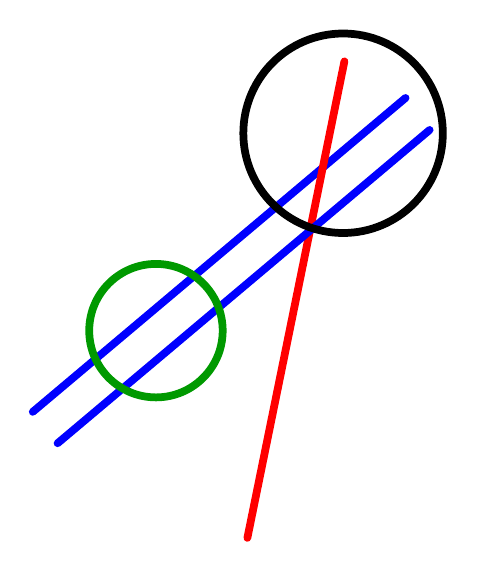
\begin{tikzpicture}[line cap=round,line join=round,>=triangle 45,x=1.0cm,y=1.0cm]
\clip(2.4,0.75) rectangle (7.75,7.3);
\draw [line width=2.8pt,color=qqqqff] (2.4644395930954643,2.4205807099751278)-- (7.199120666518885,6.4076805612790615);
\draw [line width=2.8pt,color=ffqqqq] (6.422554452918324,6.872100757665542)-- (5.190243033337279,0.8200824526119717);
\draw [line width=2.8pt,color=qqqqff] (2.7798456657281436,2.0219752974552785)-- (7.504966362216294,6.001024305024248);
\draw [line width=2.8pt] (6.405604560046194,5.959117174062875) circle (1.2667403722174913cm);
\draw [line width=2.8pt,color=qqzzqq] (4.0290654383489075,3.4521255090473444) circle (0.847551919863971cm);
%\draw [line width=2.8pt,color=qqzzqq] (5.553853552823379,2.385862623546985) circle (0.5538395445164014cm);
\end{tikzpicture}
\end{minipage}\hfill
\begin{minipage}{.5\textwidth}
\begin{center}
\quad \\
\quad \\
\includegraphics[width=.7\textwidth]{img/treestructuregeogebra_transparent}
\begin{equation}
\nonumber \mathcal{G} = \Bigl(\bigl[{\color{blue}[a]},{\color{blue}[b]},{\color{mygreen}[a,b]},{\color{red}[c]},[a,b,c]\bigr],\preceq\Bigr)
\end{equation}
\end{center}
{\flushleft E.g.:}
\begin{gather}
\nonumber [a]\preceq [a,b] \preceq [c]\\
\nonumber [a,b,c]\npreceq [c]
\end{gather}
\end{minipage}
\end{frame}


\begin{frame}
\frametitle{Nomenclature}

\begin{itemize}
\item Valid/Invalid Bundle
\begin{description}
\item[VB]: fascicle belonging to the ground truth
\item[IB]: fascicle made of false positives
\end{description}
\item Valid/Invalid Connection
\begin{description}
\item[VC]: fibre belonging to a VB
\item[IC]: fibre belonging to an IB
\end{description}
\end{itemize}
\end{frame}


\section{Formalisation}

\begin{frame}
\frametitle{The problem}
\begin{center}
\textbf{Find $x^*\in\RR^c$ such that}
\end{center}
\begin{equation}
\nonumber
x^* = \argmin_{x\in \RR^c_+}\onehalf\normtwosq{Ax-y} + \lambda \Omega(x) 
\end{equation}

\begin{center}
%\textbf{HNNLS: Hierarchical Non Negative Least Squares}
\quad \\ \quad \\
\textbf{RLS: Regularised Least Squares}
\end{center}
\end{frame}

\begin{frame}
\frametitle{Penalty term $\Omega$}
\quad \\ \quad \\
Objective:

\begin{center}
\textbf{Cancel invalid bundles}\\
$\Downarrow$\\
\textbf{Sparsity in the space of fibres}
\end{center}

\begin{minipage}{.45\linewidth}

\includegraphics[width=\linewidth]{img/norm1}
\end{minipage}\hfill
\begin{minipage}{.45\linewidth}
\begin{center}
Classical sparsity:\\ $\Omega(x) = \norm{x}_1$
\end{center}\end{minipage}
\end{frame}

\begin{frame}
\frametitle{Hierarchical sparsity}
\begin{minipage}{.25\textwidth}
\quad \\
\quad \\
\quad \\
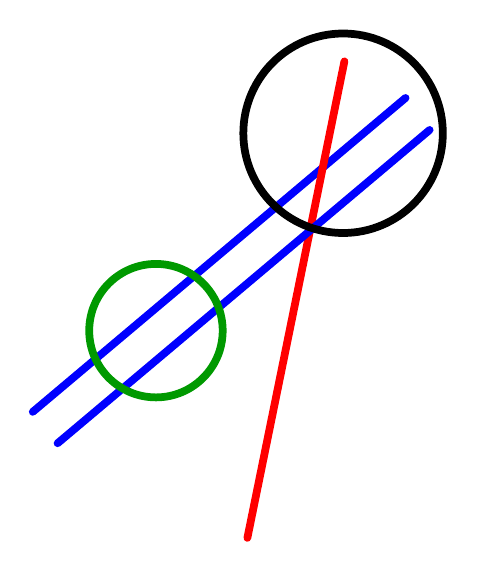
\begin{tikzpicture}[line cap=round,line join=round,>=triangle 45,x=1.0cm,y=1.0cm]
\clip(2.4,0.75) rectangle (7.75,7.3);
\draw [line width=2.8pt,color=qqqqff] (2.4644395930954643,2.4205807099751278)-- (7.199120666518885,6.4076805612790615);
\draw [line width=2.8pt,color=ffqqqq] (6.422554452918324,6.872100757665542)-- (5.190243033337279,0.8200824526119717);
\draw [line width=2.8pt,color=qqqqff] (2.7798456657281436,2.0219752974552785)-- (7.504966362216294,6.001024305024248);
\draw [line width=2.8pt] (6.405604560046194,5.959117174062875) circle (1.2667403722174913cm);
\draw [line width=2.8pt,color=qqzzqq] (4.0290654383489075,3.4521255090473444) circle (0.847551919863971cm);
%\draw [line width=2.8pt,color=qqzzqq] (5.553853552823379,2.385862623546985) circle (0.5538395445164014cm);
\end{tikzpicture}
\end{minipage}\hfill
\begin{minipage}{.5\linewidth}
\begin{equation}
\nonumber\Omega(x) = \norm{X_\mathcal{G}}_1 = \sum_{g\in\mathcal{G}}\norm{x_{|g}}_2
\end{equation}
\begin{gather}
\nonumber g = \left[a,b\right], \quad x = \left[x_a,x_b,x_c\right] \\
\nonumber \Rightarrow x_{|g} = \left[x_a,x_b,0\right]
\end{gather}

\begin{gather}
\nonumber \Omega(x) = \norm{\color{blue}[x_a,0,0]}_2 + \norm{\color{blue}[0,x_b,0]}_2 +\\
\nonumber \norm{\color{mygreen}[x_a, x_b,0]}_2 + \norm{\color{red}[0,0,x_c]}_2 +\\
\nonumber \norm{[x_a, x_b,x_c]}_2
\end{gather}
\end{minipage}
\end{frame}



\begin{frame}
\frametitle{The problem}
\begin{center}
\textbf{Find $x^*\in\RR^c$ such that}
\end{center}
\begin{equation}
\nonumber
x^* = \argmin_{x\in \RR^c}\underbrace{\onehalf\normtwosq{Ax-y}}_{\text{smooth}} + \underbrace{\lambda \Omega(x) + \iota_{\ge 0}(x)}_{\text{non smooth}}
\end{equation}

\begin{center}
\textbf{HNNLS: Hierarchical Non Negative Least Squares}
\end{center}
\end{frame}

\section{Numerical optimisation}

\begin{frame}
\frametitle{Proximal operator}
\textbf{Proximal operator of $f$:}
\begin{equation}
\nonumber \prox{f}{x} = \argmin_{y\in\RR^c} \frac{1}{2}\normtwosq{x-y} + f(y)
\end{equation}


\textbf{If $f(x) = \iota_S(x)$ with $S$ convex set:}
\begin{equation}
\nonumber \prox{f}{x} = \Pi_S(x)
\end{equation}

{\Large \begin{equation}
\nonumber
\prox{\iota_{\ge 0}}{x} = \Pi_{\ge 0}(x)
\end{equation}}
\end{frame}

\begin{frame}
\frametitle{Proximal of \,$\Omega$}
\quad \\
\textbf{Let $\mathcal{G}$ tree structure with order $\preceq$}
\begin{equation}
\nonumber
\Omega(x) = \sum_{g\in\mathcal{G}}\omega_g \norm{x_{|g}}
\end{equation}

\textbf{Compute $\prox{\Omega}{x}$}
\begin{enumerate}
\item Set $v = x$.
\item For $g\in\mathcal{G}$ following $\preceq$ do
\begin{equation}
\nonumber
v_{|g} \longleftarrow v_{|g} - \Pi_{\norm{\cdot}_*\le\omega_g}\left(v_{|g}\right).
\end{equation}
\end{enumerate}
\quad \\ \quad \\ \quad \\ \quad \\
{\footnotesize Jenatton et al., ``Proximal methods for sparse hierarchical dictionary learning'', 2010, ICML-10}
\end{frame}

\begin{frame}
\frametitle{Davis-Yin splitting scheme(2015)}
Objective:
\begin{equation}
\nonumber
x^* = \argmin_{y\in\RR^c} \overbrace{f(y)}^{\text{s}} + \overbrace{g(y) + h(y)}^{\text{ns}}
\end{equation}

Algorithm:
\begin{align}
\nonumber&y = \prox{\gamma g}{x}\\
\nonumber&z = \prox{\gamma h}{2x-y-\gamma\nabla f(y)}\\
\nonumber&x^+ = x - y + z
\end{align}



\textbf{Rate of convergence: }
\begin{equation}
\nonumber
\mathcal{O}\left(1/k\right)
\end{equation}

\end{frame}


\begin{frame}
\frametitle{Non negativity}
\quad \\
\begin{definition}[Absolute norm]
A norm $\Omega: X\to \RR$ is called \emph{absolute} if $\forall u,v\in\RR^N$ such that $|u_j|\le |v_j|$ for all $j$ implies $\Omega(u)\le \Omega(v)$.
\end{definition}

\begin{theorem}[Proximal operator of absolute norms]
Let $w\in\RR^n$ and $\lambda>0$. Consider an absolute norm $\Omega$. We have
\begin{equation}
\nonumber
\argmin_{z\in\RR^n_+}\left[\frac{1}{2}\normtwosq{w - z} + \lambda \Omega(z)\right] = \argmin_{z\in\RR^n}\left[\frac{1}{2}\normtwosq{[w]_+ - z} + \lambda \Omega(z)\right].
\end{equation}
\end{theorem}
\begin{align}
\nonumber \prox{\lambda\Omega+\iota_{\ge 0}}{w} &= \prox{\lambda\Omega}{[w]_+}\\
\nonumber &=\prox{\lambda\Omega}{\prox{\iota_{\ge 0}}{w}}
\end{align}
{\footnotesize Jenatton et al., ``Proximal methods for hierarchical sparse coding'', 2011, JMLR}
\vfill
\end{frame}


\begin{frame}
\frametitle{FISTA}
\quad \\ \quad \\
\textbf{Fast Iterative Shrinkage Thresholding Algorithm} (2009)
\quad \\ \quad \\
Objective:
\begin{equation}
\nonumber
x^* = \argmin_{x\in\RR^c} \overbrace{f(x)}^{\text{s}} + \overbrace{g(x)}^{\text{ns}}% = \argmin_{x\in \RR^c} \onehalf\normtwosq{Ax-y} + \lambda\Omega(x) + \iota_{\ge 0}(x)
\end{equation}
Algorithm ($t_0 = 1$):
\begin{align}
\nonumber &x_k = \prox{t_k g}{x_{k-1} - t_k\nabla f(x_{k-1})}\\
%p_{L}(y_{k})\\
\nonumber &t_{k+1} = \frac{1+\sqrt{1+4t_k^2}}{2}\\
\nonumber &y_{k+1} = x_k + \left(\frac{t_k-1}{t_{k+1}}\right)\left(x_k - x_{k-1}\right)
\end{align}

\textbf{Rate of convergence: }
\begin{equation}
\nonumber
\mathcal{O}\left(1/k^2\right)
\end{equation}

%\vfill%\quad \\ \quad \\ \quad \\ \quad \\
%{\tiny Beck and Teboulle., ``A fast iterative shrinkage-thresholding algorithm for linear inverse problems'', 2009}

\end{frame}

\section{Results}

\begin{frame}
\frametitle{Dataset}
\vfill
\begin{minipage}{.45\textwidth}
\includegraphics[width=\textwidth]{img/fulltract}
\end{minipage}\hfill
\begin{minipage}{.45\textwidth}
\begin{equation}
\nonumber
\normtwosq{Ax-y}
\end{equation}
\begin{itemize}
\item[$A$] Tractography:\\\quad Particle Filtering$^\text{1}$
\item[$y$] TDI map given by the fibres belonging to VBs
\end{itemize}
\end{minipage}

\quad \\ \quad \\
{\small $^\text{1}$ Girard and Descoteaux. \emph{Online filtering tractography: tracking with anatomical priors}, ISMRM 2013\\}
\end{frame}

\begin{frame}
\frametitle{Competitors}
\quad \\

\textbf{SIFT2}

Smith, Robert E., et al. "\emph{SIFT2: Enabling dense quantitative assessment of brain white matter connectivity using streamlines tractography.}" Neuroimage 119 (2015): 338-351.

\quad \\
\textbf{LiFE}

Pestilli, Franco, et al. "\emph{Evaluation and statistical inference for human connectomes.}" Nature methods 11.10 (2014): 1058-1063.

\vfill
\begin{center}
\textbf{Same goal of HNNLS}


\quad \\
No convexity, huge computational effort,\\no microstructure information, \dots
%\begin{itemize}
%\item SIFT2 doesn't cancel any bundle
%\item LiFE cancels $4$ invalid bundles
%\end{itemize}
\end{center}
\end{frame}

\begin{frame}
\frametitle{Results: Invalid Bundles (IB)}
\quad \\
\begin{center}
\includegraphics[width=.49\linewidth]{img/results/inf/ResultsIB}\hfill
\includegraphics[width=.49\linewidth]{img/results/30/ResultsIB}\\
\includegraphics[width=.49\linewidth]{img/results/20/ResultsIB}\hfill
\includegraphics[width=.49\linewidth]{img/results/10/ResultsIB}\hfill
%\includegraphics[width=.9\textwidth]{img/resultsIB}
\end{center}
\end{frame}

\begin{frame}
\frametitle{Results: Valid Bundles (VB)}
\quad \\
\begin{center}
\includegraphics[width=.49\linewidth]{img/results/inf/ResultsVB}\hfill
\includegraphics[width=.49\linewidth]{img/results/30/ResultsVB}\\
\includegraphics[width=.49\linewidth]{img/results/20/ResultsVB}\hfill
\includegraphics[width=.49\linewidth]{img/results/10/ResultsVB}\hfill
%\includegraphics[width=.9\textwidth]{img/resultsIB}
\end{center}
\end{frame}

\begin{frame}
\frametitle{Results}
{\small \begin{multline}
\nonumber
\lambda \in \big\{
\begin{array}{cccccccc}
0 & 0.012 & 0.020 & 0.035 & 0.059 & 0.100 & 0.168 & 0.284
\end{array}
\\
\begin{array}{cccccccc}
0.480 & 0.809 & 1.364 & 2.300 & 3.879 & 6.540 & 11.02 & 18.59
\end{array}
\big\}
\end{multline}}
\begin{tabular}{|c|c|c|c|c|c|c|c|c|c|}
\hline 
&SIFT2 & LiFE & $\lambda=0$ & $\lambda_1$ & $\lambda_2$ & $\lambda_3$ & $\lambda_4$ & $\lambda_5$ & $\lambda_6$ \\
\hline 
VB&25 & 25 & 25 & 25 & 25 & 25 & 25 & 25 & 25 \\
\hline 
IB&427 & 423 & 284 & 205 & 184 & 162 & 138 & 115 & 95\\
\hline 
\hline
& $\lambda_7$ & $\lambda_8$ & $\lambda_9$ & $\lambda_{10}$ & $\lambda_{11}$ & $\lambda_{12}$ & $\lambda_{13}$ & $\lambda_{14}$ & $\lambda_{15}$\\ 
\hline 
VB & 25 & 25 & 25 & 25 & 25 & 25 & 25 & 24 & 23\\
\hline 
IB & 71 & 56 & 42 & 33 & 19 & 11 & 5 & 1 & 0\\
\hline 
\end{tabular}
\end{frame}

\begin{frame}
\frametitle{Results: Kept fibres}
\quad \\
\begin{center}
\includegraphics[width=.49\linewidth]{img/results/inf/ResultsPERC}\hfill
\includegraphics[width=.49\linewidth]{img/results/30/ResultsPERC}\\
\includegraphics[width=.49\linewidth]{img/results/20/ResultsPERC}\hfill
\includegraphics[width=.49\linewidth]{img/results/10/ResultsPERC}\hfill
%\includegraphics[width=.9\textwidth]{img/resultsIB}
\end{center}
\end{frame}

\begin{frame}
\frametitle{Results: Valid Connections}
\quad \\
\begin{center}
\includegraphics[width=.49\linewidth]{img/results/inf/ResultsPROP}\hfill
\includegraphics[width=.49\linewidth]{img/results/30/ResultsPROP}\\
\includegraphics[width=.49\linewidth]{img/results/20/ResultsPROP}\hfill
\includegraphics[width=.49\linewidth]{img/results/10/ResultsPROP}\hfill
%\includegraphics[width=.9\textwidth]{img/resultsIB}
\end{center}
\end{frame}

%
%
%\begin{frame}
%\frametitle{Results: Valid Bundles (VB)}
%\begin{center}
%\includegraphics[width=.9\textwidth]{img/resultsVB}
%\end{center}
%\end{frame}
%
%\begin{frame}
%\frametitle{Overall performance}
%\begin{center}
%\includegraphics[width=.85\textwidth]{img/resultsoverall}
%\end{center}
%\end{frame}


\section{Future work}
\begin{frame}
\frametitle{Still to be done...}
\vfill
\begin{itemize}
\item Sensitivity analysis w.r.t. tractogram
\item Sensitivity analysis w.r.t. clustering thresholds
\item Set up a strategy for selecting $\lambda$
\item Exploit more sophisticated solvers (Canales, 2015)
\end{itemize}
\vfill
\end{frame}

\begin{frame}
\frametitle{Thank you}

\quad \\

\begin{center}
\includegraphics[width=\textwidth,height=.8\textheight]{img/wordcloudtesi}
\end{center}
\end{frame}

\appendix
\backupbegin
\section{Backup}

\begin{frame}
\frametitle{Reweighted $\ell_1$}
Objective:

\begin{center}
\textbf{Smart choice of $w_g$}
\end{center}

Iteratively define
\begin{equation}
\nonumber w_g = \frac{1}{\norm{x_g}_1+\epsilon}
\end{equation}
and restart the optimisation procedure.
\quad \\ \quad \\
{\tiny Candes, Emmanuel J., Michael B. Wakin, and Stephen P. Boyd. "Enhancing sparsity by reweighted l1 minimization." Journal of Fourier analysis and applications, 2008}
\end{frame}


\begin{frame}
\frametitle{RUMBA}
\begin{center}
\textbf{Robust and Unbiased Model-Based Spherical Deconvolution}
\end{center}
\begin{gather}
\nonumber\prob\left(S_i|\bar{S}_i, \sigma^2,n\right) = \frac{\bar{S}_i}{\sigma^2}\left(\frac{S_i}{\bar{S}_i}\right)^n \exp\left\{-\frac{1}{2\sigma^2}\left[S_i^2+\bar{S}_i^2\right]\right\}I_{n-1}\left(\frac{S_i\bar{S}_i}{\sigma^2}\right)u(S_i),\\
\nonumber f = f\circ \frac{H^t\left[S\circ\frac{I_n(S\circ Hf/\sigma^2)}{I_{n-1}(S\circ Hf/\sigma^2)}\right]}{H^tHf}
\end{gather}
where $S_i = \left(Hf\right)_i$.

\quad \\ \quad \\
{\small Canales-Rodríguez, Erick J., et al. \emph{Spherical deconvolution of multichannel diffusion MRI data with non-Gaussian noise models and spatial regularization.} PloS one 10.10 (2015).}
\end{frame}

\begin{frame}[fragile]
\frametitle{Software}
\vfill
\begin{itemize}
\item Microstructure Informed Tractography
\begin{itemize}
\item COMMIT $^*$
\item HNNLS $^\ddagger$
\end{itemize}
\item Clustering
\begin{itemize}
\item Tract Querier$^\dagger$
\item QuickBundlesX$^{\ddagger\lozenge}$
\end{itemize}

\end{itemize}

\vfill

\begin{itemize}
\item[$^*$]\verb|github.com/daducci/COMMIT|
\item[$^\dagger$]\verb|github.com/demianw/tract_querier|
\item[$^\ddagger$]\verb|github.com/matteofrigo/COMMIT_demo|
\item[$^\lozenge$]\verb|github.com/MarcCote/dipy/|
\end{itemize}

\end{frame}


\backupend
\end{document}